% Chapter: The Limits of a Rating. Primer, then measure -> localize ->
% watch -> explain. Artifacts under results/elo_duel/ and results/archetypes/.

\section{Primer: rankings as altitude, cycles as the obstruction}
\label{sec:rank-primer}

Chapter~\ref{ch:ladder} compressed 312 games into one number per bot and
promised that was mostly harmless. This section builds the machinery to say
\emph{how} harmless --- slowly, on a three-bot toy, because once the
pictures are in place the real measurements read themselves.

\paragraph{A tournament is arrows with weights.} Draw the models as nodes.
For each pairing, draw one arrow from the stronger to the weaker, weighted
by the \emph{advantage}: the score rate minus $\tfrac12$. An advantage of
$0.25$ means ``wins three games in four''; an advantage of $0$ means the
pairing is even. This weighted arrow diagram --- and nothing else --- is
what any rating must summarize.

\paragraph{When does a ranking tell the whole story?} A ranking assigns
each model an \emph{altitude} $s_i$ (in the same score-rate units), and it
explains the tournament perfectly if every advantage is exactly the
altitude drop:
\[
  Y_{ij} \;=\; s_i - s_j
  \qquad\text{(``troops roll downhill'', but for bots).}
\]
Figure~\ref{fig:rank-primer}a shows such a tournament: A sits $0.3$ above
B, B sits $0.3$ above C, and --- forced by the altitudes --- A's advantage
over C is exactly $0.6$. In a perfectly rankable world, knowing the ladder
means knowing every matchup.

\paragraph{The obstruction is a loop.} Altitude drops telescope: walking
any closed loop, the drops must sum to zero --- you cannot hike downhill
all the way around a mountain. So a rock-paper-scissors triangle
(Figure~\ref{fig:rank-primer}b), where each model holds a $+0.25$ advantage
over the next, is not explainable by \emph{any} altitudes whatsoever: the
loop gains $+0.75$. Cycles are not badly-ranked data; they are data that no
ranking, however cleverly fit, can represent.

\paragraph{Every tournament splits into the two.} The general case mixes
both ingredients, and the split is clean
(Figure~\ref{fig:rank-primer}c). Recover each model's altitude as its
\emph{average advantage over the field} (on a full round-robin this is the
least-squares fit); subtract the altitude drops from the arrows; what
remains circulates in loops with nothing left over. In the worked example,
a tournament with advantages $0.4/0.1/0.2$ splits into an altitude part
($0.3/0/0.3$: A well above B and C, those two tied) plus a pure loop of
strength $0.1$. This is the Hodge decomposition of ranking data
\citep{jiang2011}; on a complete round-robin the two parts are orthogonal,
so the tournament's total ``energy'' (sum of squared advantages) splits
exactly into an altitude share and a loop share. \textbf{The altitude share
is the number we are after: it is how rankable the game is}, and one minus
it is the fraction of competitive structure that every possible rating ---
Elo included --- must discard.

\begin{figure}[htbp]
\centering
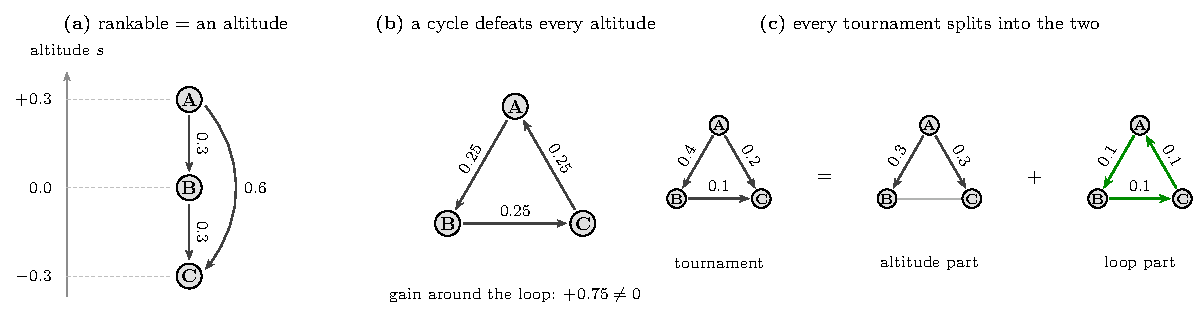
\includegraphics[width=\textwidth]{figs/rank_primer/rank_primer.pdf}
\caption{The primer on a three-bot toy. (a) A perfectly rankable
tournament \emph{is} an altitude assignment: every arrow's weight is its
altitude drop. (b) A cycle defeats every altitude: the loop gains $+0.75$,
and drops must sum to zero around any loop. (c) The general tournament
splits exactly into an altitude part plus a loop part (worked numbers;
green = the loop).}
\label{fig:rank-primer}
\end{figure}

\paragraph{Reading the loop part as a map.} One more tool and the chapter's
figures will all make sense. The loop part may contain many overlapping
cycles; it can be organized because a pure circulation is a
\emph{rotation}, and a rotation decomposes into independent planes, ordered
by how much circulation each carries. Projecting the models onto the
\emph{leading} plane \citep{balduzzi2019} draws a map of the dominant
cycle, and the map is read in polar coordinates: a model's \textbf{angle}
is its position in the cycle (following angles around the circle reads out
the who-beats-whom order), and its \textbf{radius} is how strongly it
participates (models at the center sit outside the cycle entirely). The
axes themselves carry no meaning individually --- only angle and radius do.

\paragraph{The plan.} With the pictures in place, the chapter now: measures
the altitude/loop split for CRisky's tournaments (\S\ref{sec:elo-hodge});
draws the leading-plane map and finds the cycle is organized by strategic
posture (\S\ref{sec:elo-cycles}); watches the cycle turn in a single
replayed game (\S\ref{sec:elo-podium}); and tests a proposed mechanism for
it with controlled archetypes (\S\ref{sec:elo-rps}).

\section{Measuring: how rankable is CRisky?}
\label{sec:elo-hodge}

The question, now precise: what fraction of the tournament's energy does
the altitude part carry? The answer: \textbf{\hodgetransitivityduel} in the
duel tournament, \hodgetransitivity{} in the free-for-all ---
\textbf{roughly a fifth of the game is cyclic under either protocol}. Two
consequences follow.

First, the intransitivity is a property of the \emph{game}, not the seating
arrangement: two very different competitive environments produce the same
loop share. Second, Elo is not the culprit. The recovered altitude agrees
with the Bradley--Terry rating on the order of all thirteen models exactly
(Spearman $\rho = \hodgespearmanduel$; Figure~\ref{fig:hodge}), so no
cleverer scalar fit would do better --- the missing fifth is invisible to
one-dimensional summaries as a class. The full pairwise data is therefore
summarized without loss by exactly two objects: the altitude
(Table~\ref{tab:elo}) and the loops, to which we now turn.

\begin{figure}[htbp]
\centering

\includegraphics[width=0.62\textwidth]{\resultsfig{elo_duel/figures/hodge_vs_elo.pdf}}
\caption{The two scalar summaries agree. Horizontal axis: each model's
recovered altitude $s_i$ --- its average advantage over the field, in
score-rate units (\S\ref{sec:rank-primer}). Vertical axis: its
Bradley--Terry rating from Chapter~\ref{ch:ladder}. The relationship is
monotone ($\rho = \hodgespearmanduel$), so the two ranking methods tell one
story; the chapter's subject is the \hodgecurlduel{} of the tournament that
neither can hold.}
\label{fig:hodge}
\end{figure}

\section{Localizing: one cycle, organized by posture}
\label{sec:elo-cycles}

Is the cyclic fifth diffuse noise --- a little circulation everywhere ---
or does it have a shape? Decomposing the loop part into its rotation
planes (\S\ref{sec:rank-primer}) gives a sharp answer: \textbf{the leading
plane alone carries \cycleplaneshareduel{} of the loop energy}. To a first
approximation, CRisky has \emph{one} game-wide cycle
(Figure~\ref{fig:cyclic-plane}).

And the cycle has legible structure: reading angles around the map, the
models cluster by strategic posture --- the war-first knapsack models sit
together (0--40$^\circ$), the OT podium together (88--116$^\circ$), the
economy-first mid-table together (180--250$^\circ$). Whatever generates the
intransitivity moves \emph{families} of models around the wheel together,
which is the first hint that posture itself is the mechanism --- the
hypothesis \S\ref{sec:elo-rps} puts to a controlled test.

\begin{figure}[htbp]
\centering

\includegraphics[width=0.6\textwidth]{\resultsfig{elo_duel/figures/cyclic_plane.pdf}}
\caption{The dominant cycle, mapped: models projected onto the leading
rotation plane of the duel tournament's loop part. Read in polar
coordinates per \S\ref{sec:rank-primer}: angle = position in the cycle,
radius = strength of participation; the axes have no individual meaning.
Posture families cluster in angle.}
\label{fig:cyclic-plane}
\end{figure}

\begin{table}[htbp]
\centering
\resultstable{elo_duel/tables/curl_triangles}
\caption{The largest individual loops (circulation around each 3-cycle, in
score-rate units; $\pm\tfrac32$ is the maximum possible). The podium itself
is near-cyclic in head-to-head play: \code{v9} takes \code{v8} 0.75,
\code{v12} takes \code{v9} 0.75, \code{v12}--\code{v8} splits.}
\label{tab:curl}
\end{table}

\section{Watching: the podium cycle in a single game}
\label{sec:elo-podium}

Statistics established the cycle; a replay shows what it looks like on the
map. The podium's head-to-head structure cycles under both protocols
(Table~\ref{tab:curl}), and Figure~\ref{fig:v9v8} replays FFA tournament
game 1272 (\code{v8} in the test seat vs.\ two independent \code{v9}). The
game is decided almost immediately: \code{v8} expands fastest off the start
--- peaking near 75 nodes by tick 250 --- but is torn apart in the first
contact wars and eliminated by tick $\sim$600. Everything after is the two
\code{v9} seats partitioning the map (the solid copy plateaus around 240
nodes and wins the node count at timeout). Two lessons. First, losses in
this game are not slow grinds but \emph{early-war collapses} --- a pattern
that recurs in every case study in this report and explains why fast-payoff
economies beat gym-optimal ones (\S\ref{sec:economy}). Second, whatever
edge \code{v8}'s local softmax buys against the field, it does not survive
simultaneous pressure from two OT-supplied fronts: the cycle is real, and
it turns on \emph{which} strength a matchup happens to probe.

\begin{figure}[htbp]
\centering

\includegraphics[width=\textwidth]{\resultsfig{case_studies/figures/v9_beats_v8.pdf}}
\caption{FFA tournament game 1272 replayed. All three curves are the three
players of this \emph{single} game: \code{v8} in the test seat (blue) and
the two independent \code{v9} instances (green, solid/dashed). Left: total
troops; right: nodes held. After \code{v8}'s elimination the remaining
dynamics are the two \code{v9} seats fighting each other.}
\label{fig:v9v8}
\end{figure}

\section{Explaining: testing the rock--paper--scissors hypothesis}
\label{sec:elo-rps}

The posture clustering of \S\ref{sec:elo-cycles} begs for a mechanism, and
there is a candidate on the table (Joel's, predating these experiments):
the game maps onto rock--paper--scissors by strategic posture.
\emph{Rock} = aggressive; \emph{paper} = defensive but distrustful (stacks
borders); \emph{scissors} = defensive and trusting (just builds).
Predicted: rock $>$ scissors (steamroll), scissors $>$ paper (leaner
allocation), paper $>$ rock (defender's advantage). If true, this names
the wheel of \S\ref{sec:elo-cycles}.

The nearest existing models
(\code{v1\_knapsack}/\code{v0\_expansion}/\code{v12}) cannot test it ---
they differ in chassis quality (economy, transport era), and indeed that
triple is perfectly transitive in both tournaments (\code{v12} $>$ \code{v0}
$>$ \code{v1k}, 8/8 each): power differences drown posture. So we built
three archetypes on \emph{one} chassis (v12's QUBO economy + OT transport,
\code{src/ai/models/archetypes.cpp}) differing only in posture, and played
the triangle (12 duels per pair, Table~\ref{tab:archetypes}).

\begin{table}[htbp]
\centering
\resultstable{archetypes/tables/archetypes}
\caption{Archetype triangle, posture isolated on a fixed chassis. Score rate
is for the first-named archetype.}
\label{tab:archetypes}
\end{table}

Two of three edges confirm the theory --- rock sweeps scissors 12/12
(steamroll), paper sweeps rock 12/12 (defender's advantage) --- but the
linchpin edge fails: \textbf{paper also sweeps scissors 12/12, so there is
no cycle; border-stacking dominates}. The diagnosis is mechanical: in the
current rules, parked troops cost \emph{nothing} --- they are not consumed,
do not decay, and do not reduce production --- so ``resources more
efficiently allocated to building'' never cashes out. (One caveat: our
paper archetype still launches attacks when it sees a guaranteed win ---
the knob we turned down governs where troops gather, not whether attacks
fire --- so a purist test awaits an attack-suppression switch.)

This closes the chapter's arc, and ties the report's threads together. The
posture wheel is two-thirds real, and its missing edge is a statement about
the \emph{game}, not the bots: standing armies are free. The same fact
appears twice more in this report --- the border reserve is what rescues
\code{v11} into \code{v12} (\S\ref{sec:elo-v11}), and what sweeps the
corridor map (\S\ref{sec:combat}). Under the current rules, border-stacking
is simply the dominant posture; give garrisons a cost (upkeep, or
production diverted) and the RPS wheel plausibly activates
(Chapter~\ref{ch:findings}). The intransitivity that exists \emph{today}
lives higher in the stack: the podium's softmax-vs-transport cycle, where
the strengths being probed differ by matchup rather than by posture.
